\documentclass[12pt]{article} % use larger type; default would be 10pt
\usepackage[czech]{babel}
\usepackage[utf8]{inputenc} % set input encoding (not needed with XeLaTeX)

%%% PAGE DIMENSIONS
\usepackage{geometry} % to change the page dimensions
% \usepackage[left=2cm,right=2cm,top=2cm,bottom=2cm]{geometry}
\geometry{a4paper}
% \geometry{margin=2in} % for example, change the margins to 2 inches all round
% \geometry{landscape} % set up the page for landscape

\usepackage{graphicx} % support the \includegraphics command and options
\usepackage{wrapfig} % support the wrapfigure section

\usepackage{hyperref} % links in \tableofcontents
\hypersetup{
	colorlinks,
	citecolor=black,
	filecolor=black,
	linkcolor=black,
	urlcolor=black
}

% \usepackage[parfill]{parskip} % Activate to begin paragraphs with an empty line rather than an indent

%%% PACKAGES
\usepackage{booktabs} % for much better looking tables
\usepackage{array} % for better arrays (eg matrices) in maths
%\usepackage{paralist} % very flexible & customisable lists (eg. enumerate/itemize, etc.)
\usepackage{verbatim} % adds environment for commenting out blocks of text & for better verbatim
\usepackage{subfig} % make it possible to include more than one captioned figure/table in a single float
% These packages are all incorporated in the memoir class to one degree or another...
\usepackage{tikz} % graphs
\usepackage{pgfplots}
\usepackage{float}

%%% HEADERS & FOOTERS
\usepackage{fancyhdr} % This should be set AFTER setting up the page geometry
\pagestyle{fancy} % options: empty , plain , fancy
\renewcommand{\headrulewidth}{0pt} % customise the layout...
\lhead{}\chead{}\rhead{}
\lfoot{}\cfoot{\thepage}\rfoot{}

%%% SECTION TITLE APPEARANCE
\usepackage{sectsty}
\allsectionsfont{\sffamily\mdseries\upshape} % (See the fntguide.pdf for font help)
% (This matches ConTeXt defaults)

%%% ToC (table of contents) APPEARANCE
\usepackage[nottoc,notlof,notlot]{tocbibind} % Put the bibliography in the ToC
\usepackage[titles,subfigure]{tocloft} % Alter the style of the Table of Contents
\renewcommand{\cftsecfont}{\rmfamily\mdseries\upshape}
\renewcommand{\cftsecpagefont}{\rmfamily\mdseries\upshape} % No bold!
\newcommand{\bigsize}{\fontsize{35pt}{20pt}\selectfont}

%%% END Article customizations

\begin{document}
\begin{titlepage}
	
\includegraphics[scale=0.7]{logo.jpg}
	\vspace*{\fill}
	\begin{center}
		\textsc{\LARGE Měření kmitočtu a časových\\intervalů čítačem}\\[1cm]
		Martin Zlámal \\[1cm]
		{\small\em \ Datum měření 26. listopadu 2013 } \\
		{\small\em \copyright \ Datum poslední revize \today } \\
		\LaTeX
	\end{center}
	\vspace*{\fill}
\end{titlepage}
%\tableofcontents
%\listoffigures
%\listoftables
\newpage

\section{Zadání}
\begin{enumerate}
\item Změřte kmitočet, periodu a časové intervaly pro 3 různé nastavení generátoru
v rámci jednoho rozsahu.
\item Výsledky porovnejte mezi sebou a měřením pomocí osciloskopu.
\item Nacejchujte generátor z hlediska kmitočtu na jednom rozsahu. Určete korekci a
nakreslete korekční křivku. Vypočtěte chybu měření čítače.
\end{enumerate}

\section{Schéma zapojení}
\begin{figure}[H]
\center
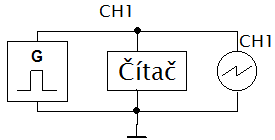
\includegraphics[scale=1]{schema.png}
\caption{Reálné schéma zapojení}
\end{figure}

\section{Naměřené a vypočítané hodnoty}
\begin{table}[H]
\caption{Naměřené hodnoty pro tři různá nastavení generátoru}
\begin{tabular}{|c|c|c|c|c|c|c|}
\hline 
Frekvence $[Hz]$ & $T\,[ms]$ & $t_{on}\,[ms]$ & $t_{off}\,[ms]$ & $T_{osc}\,[ms]$ & $t_{on-osc}\,[ms]$ & $t_{off-osc}\,[ms]$ \\ 
\hline 
$50,01$ & $20,17$ & $6,32$ & $14,20$ & $20,0$ & $6,0$ & $14,0$ \\ 
\hline 
$100,37$ & $9,96$ & $7,92$ & $2,13$ & $9,92$ & $6,96$ & $2,96$ \\ 
\hline 
$500,92$ & $1,997$ & $1,398$ & $0,601$ & $2,0$ & $1,4$ & $0,6$ \\ 
\hline 
\end{tabular} 
\end{table}

\begin{table}[H]
\caption{Nastavená a reálné frekvence pro cejchování generátoru v obou směrech}
\begin{tabular}{|c|c|c|c|c|c|c|c|c|c|}
\hline 
Frekvence & $1\,Hz$ & $2\,Hz$ & $3\,Hz$ & $4\,Hz$ & $5\,Hz$ & $6\,Hz$ & $7\,Hz$ & $8\,Hz$ & $9\,Hz$ \\ 
\hline 
Nahoru $[Hz]$ & 0,99 & 1,95 & 2,98 & 3,96 & 4,95 & 5,95 & 7,01 & 8,09 & 9,17 \\ 
\hline 
Dolů $[Hz]$ & 0,97 & 1,99 & 2,98 & 3,98 & 4,94 & 5,92 & 7,00 & 8,10 & 9,19 \\ 
\hline 
Průměr $[Hz]$ & 0,98 & 1,97 & 2,98 & 3,97 & 4,945 & 5,935 & 7,005 & 8,095 & 9,18 \\ 
\hline
\end{tabular} 
\end{table}

Absolutní a relativní chyba měřeného kmitočtu:
\begin{equation}
\Delta_f = f_s - f_g = 9,18 - 9,00 = 0,18\,Hz
\end{equation}
\begin{equation}
\delta_f = \frac{\Delta_f}{f_s}\cdot 100 = \frac{0,18}{9,18}\cdot 100 = 1,96\,\%
\end{equation}

\section{Grafy}
\begin{figure}[H]
\centering
	\begin{tikzpicture}
		\begin{axis}[
			width=0.9\textwidth,
	      	height=0.4\textwidth,
			xlabel={$f\,[Hz]$},
			ylabel={$korekce\,[Hz]$}]
		\addplot[color=blue,dashed] coordinates {
			(1,0)
			(9,0)
		};
		\addlegendentry{ideální}
		\addplot[color=red,mark=x] coordinates {
			(1,-0.02)
			(2,-0.03)
			(3,-0.02)
			(4,-0.03)
			(5,-0.055)
			(6,-0.065)
			(7,0.005)
			(8,0.095)
			(9,0.18)
		};
		\end{axis}
	\end{tikzpicture}
	\caption{Korekční křivka}
\end{figure}

\section{Závěr}
Z naměřených hodnot je vidět, že osciloskop zobrazuje měřené veličiny s menší přesností, než čítač. Toto se týká všech frekvencí. Největší rozpor mezi čítačem a osciloskopem je při nejmenší měřené frekvenci $50\,Hz$. Naopak nejvíce souhlasí hodnoty pro vysokou frekvenci $500\,Hz$.

Z korekční křivky generátoru funkcí je vidět, že generátor poměrně přesně drží nízké frekvence z měřeného rozsahu, ale pro větší frekvence již odchylka téměř plynule narůstá.

\section{Přístroje}
\begin{itemize}
\item Generátor funkcí Zopan KZ1405, evid. 127740
\item Čítač E8 FC-7015U, evid. 109723
\item Osciloskop DSO1002A, evid. 203111
\end{itemize}

\end{document}
